% Chapter 1

\chapter{Introduction} % Write in your own chapter title
\label{Chapter2}
\lhead{Chapter 2. \emph{Background and Related Work}}


\section{Basics of Artificial Neural Networks}

Artificial neurons were introduced as information processing devices more than fifty years ago\citep{mcculloch1943logical}. Following the early work, perceptrons were deployed in layers to do pattern recognition job. A lot of resource was invested in researching capability of learning perceptrons theoretically and experimentally. As shown in Figure 2.1, a neuron computes a weighted summation of its n inputs and then thresholds the result to give a binary output y. We can treat n input as an vector with n elements, and represent the vector as either class A(for output +1) or class B(for output -1).

\graphicspath{ {./Figures/} }
\begin{figure}
\begin{center}
%\fbox{\rule{0pt}{2in} \rule{0.9\linewidth}{0pt}}
   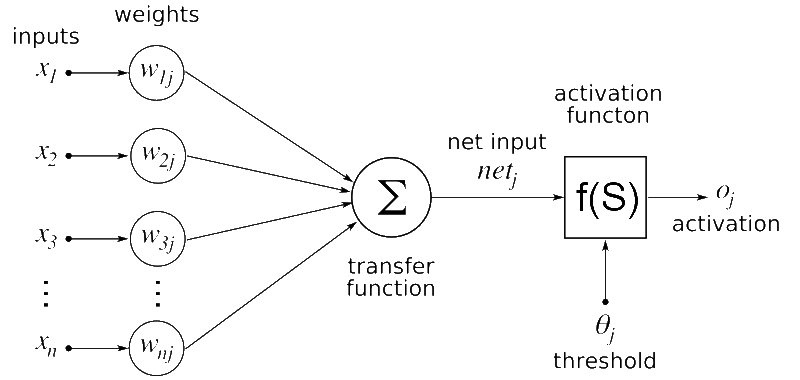
\includegraphics[width=0.8\linewidth]{Figure2-1.png}

\end{center}
   \caption{Diagram of a neuron}
\label{fig:long}
\label{fig:onecol}
\end{figure}


\section{Statistical Pattern Recognization}

In the statistical approach, the pattern is represented in terms of d dimensional feature vector and each element of the vector describes some subjects of the example. In brief, three components are essential to do statistical pattern recognization. First is a representation of the model. Second is an objective function used to evaluating the accuracy of the model. Third is an optimization method for learning a model with minimum errors.

\section{Artificial Neural Networks}

Artificial neural networks(ANNs) were proposed in the mid-20th century. The term is inspired by the structure of neural networks in the brain. It is one of the most successful statistical learning models used to approximate functions. Learning with ANNs yields an effective learning paradigm and has achieved cutting-edge performance in computer vision. 

The single-layer perceptron  has shown great success for a simple model. For increasing complex models and applications, multi-layer perceptron has exhibited the power of features learning. With hardware developing At the same time, the demanding of more efficient optimizing and model evoluation methods is needed for BIG DATA. 

Recent development in ANNs approaches have giantly advanced the performance of state-of-the-art visual recognition systems. With implementing deep convolutional neural networks, it achieves top accuracy in ImageNet Challenge. The model has been used in related fields and succeeds in competition.

\section{Weather Classification}

Weather classification is an important job in daily life. In this thesis, we are focused on two class weather conditions, sunny and cloudy. 

There are some obstacles in front of weather classification. First, because inputting pixels are independent and high dimension, say a 500x500 RPG image means 750000 pixels, computation is huge. Second, some simple middle level image characters are difficult to machines, like light, shading, sun shine. It is still not easy to detect these characters with high accuracy.  Thirdly, there are no decisive features, for example brightness and lightness, to classify scene. For example, sun shine can be both found in sunny and cloudy weather. Last but not least, outdoor images are various background.


